\documentclass[12pt,aspectratio=169]{beamer}
\usepackage{amsmath,amssymb,booktabs}
\usepackage{tikz,pgfplots}
\pgfplotsset{compat=1.18}
\usetikzlibrary{arrows.meta,positioning}

% ---- look of ch06v2 / ch07v2 ----
\setbeamertemplate{navigation symbols}{}
\definecolor{titlebg}{RGB}{214,214,240}
\definecolor{blocktitlebg}{RGB}{204,204,236}
\definecolor{blockbodybg}{RGB}{239,239,249}
\setbeamercolor{frametitle}{fg=black,bg=black!5}
\setbeamerfont{frametitle}{series=\bfseries,size=\large}
\setbeamercolor{title}{fg=black,bg=titlebg}
\setbeamerfont{title}{series=\bfseries,size=\LARGE}
\setbeamerfont{subtitle}{series=\bfseries,size=\large}
\setbeamercolor{block title}{fg=black,bg=blocktitlebg}
\setbeamercolor{block body}{fg=black,bg=blockbodybg}
\setbeamerfont{block title}{series=\bfseries}
\setbeamercolor{alerted text}{fg=red!80!black}
\setbeamertemplate{frametitle}{%
  \nointerlineskip
  \begin{beamercolorbox}[wd=\paperwidth,ht=2.6ex,dp=1.2ex,leftskip=.3cm]{frametitle}
    \usebeamerfont{frametitle}\insertframetitle
  \end{beamercolorbox}}
\setbeamertemplate{footline}{%
  \leavevmode\hbox to \paperwidth{\hskip.3cm
    {\tiny\color{black!55}\insertsectionhead\hfill\insertframenumber\,/\,\inserttotalframenumber}\hskip.3cm}
  \vskip2mm}
\setbeamertemplate{title page}{%
  \vfill
  \begin{beamercolorbox}[wd=\textwidth,sep=8pt,center]{title}
    {\usebeamerfont{title}\inserttitle\par}\vskip3pt
    {\usebeamerfont{subtitle}\insertsubtitle\par}
  \end{beamercolorbox}
  \vskip1.2em
  \begin{center}
    \insertauthor\par\vskip.8em
    {\small\insertinstitute}\par\vskip.8em
    \insertdate\par\vskip2em
    Reading: Nocedal \& Wright, \emph{Numerical Optimization}, 2nd ed., Chapter 9
  \end{center}
  \vfill}

\newcommand{\readpp}[1]{{\color{red!80!black}\textbf{Read:} #1}}
\newcommand{\eps}{\epsilon}
\newcommand{\R}{\mathbb{R}}
\newcommand{\xb}{\bar x}

\title{Advanced Optimization}
\subtitle{Chapter 9 --- Derivative-Free Optimization}
\author{Hongseok Kim}
\institute{Department of Electronic Engineering, Sogang University}
\date{Fall 2026}

\newcommand{\algblock}[1]{\begin{block}{}#1\end{block}}
\newcommand{\kw}[1]{\textbf{#1}}
\newcommand{\ind}{\hspace*{1.2em}}

\begin{document}

\section{Chapter 9: introduction}

\begin{frame}
  \titlepage
\end{frame}

\begin{frame}{When derivatives are not available}
  Typical situations:
  \begin{itemize}
    \item $f(x)$ is an experimental measurement or a stochastic simulation.
    \item $f$ is given only as binary code, or as code in several languages: AD (Chapter 8) cannot be applied.
    \item Coding the derivatives is too time consuming.
  \end{itemize}
  \begin{block}{The idea}
    Do not approximate the gradient. Use $f$ at a set of \alert{sample points} to choose the next iterate.
  \end{block}
  Methods: model-based (\S9.2), coordinate and pattern search (\S9.3), conjugate directions (\S9.4),
  Nelder--Mead (\S9.5), implicit filtering (\S9.6). Not treated: simulated annealing.
\end{frame}

\begin{frame}{Scope of this chapter}
  \begin{equation}
    \min_{x\in\R^n} f(x) \tag{9.1}
  \end{equation}
  \begin{itemize}
    \item Unconstrained, and $f$ has a continuous derivative that we cannot compute.
    \item DFO methods are less developed than gradient-based methods:
      \alert{effective only for small problems}.
    \item DFO methods are often used, with mixed success, for nonsmooth or global problems.
      These are outside the scope of the book.
    \item Noise is treated in \S9.1 and \S9.6.
  \end{itemize}
  \readpp{pp.~220--221.}
\end{frame}

\section{\S9.1 Finite differences and noise}

\begin{frame}{Noisy function values}
  The obvious approach: finite-difference gradient + a gradient-based method.
  It should always be considered, but noise can ruin it.
  Noise: finite simulation trials, solver tolerances.
  \begin{equation}
    f(x) = h(x)+\phi(x), \qquad h \text{ smooth},\ \phi \text{ noise}. \tag{9.2}
  \end{equation}
  Central difference (8.7) with interval $\eps$, and the noise level on the box around $x$:
  \begin{align}
    \nabla_\eps f(x) &= \left[\frac{f(x+\eps e_i)-f(x-\eps e_i)}{2\eps}\right]_{i=1,\dots,n}, \tag{9.3}\\
    \eta(x;\eps) &= \sup_{\|z-x\|_\infty\le\eps}|\phi(z)|. \tag{9.4}
  \end{align}
\end{frame}

\begin{frame}{Lemma 9.1: truncation versus noise}
  \begin{block}{Lemma 9.1}
    Suppose that $\nabla^2 h$ is Lipschitz continuous in a neighborhood of the box
    $\{z \mid \|z-x\|_\infty\le\eps\}$ with Lipschitz constant $L_h$. Then
    \begin{equation}
      \|\nabla_\eps f(x)-\nabla h(x)\|_\infty \le L_h\eps^2 + \frac{\eta(x;\eps)}{\eps}. \tag{9.5}
    \end{equation}
  \end{block}
  \begin{itemize}
    \item Same argument as for (8.5), with roundoff replaced by noise (Exercise 9.1).
    \item If $\eta$ dominates $\eps$, the estimate has no accuracy at all.
      Then $-\nabla_\eps f$ is a descent direction only by luck.
    \item Alternative: spread the sample points more widely and build a \alert{model} of $f$.
  \end{itemize}
  \readpp{pp.~221--223.}
\end{frame}

\begin{frame}{Numerical example: noise moves the best $\eps$}
  \begin{columns}[T]
    \begin{column}{.56\textwidth}
      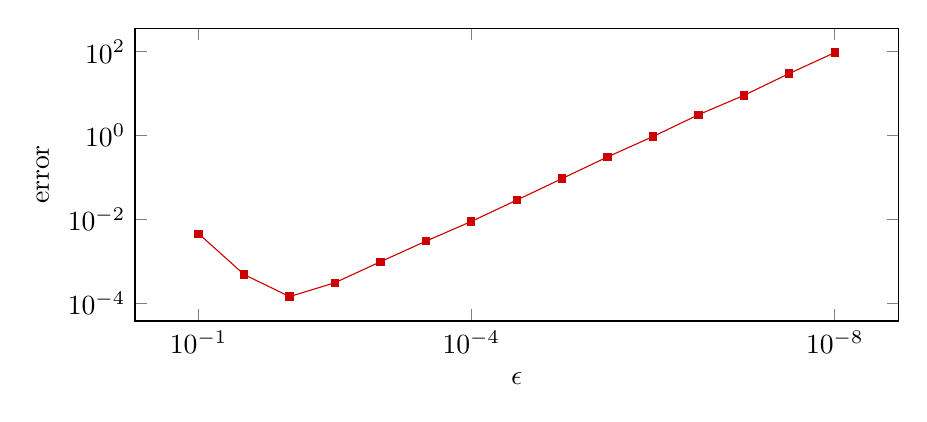
\begin{tikzpicture}
        \begin{loglogaxis}[width=.93\linewidth,height=5.3cm,
            xlabel={$\eps$},ylabel={error},x dir=reverse,
            xtick={1e-1,1e-4,1e-8},ytick={1e-4,1e-2,1e0,1e2}]
          \addplot[red!80!black,mark=square*,mark size=1.3pt] coordinates {
            (1.00e-01,4.542e-03)(3.16e-02,4.822e-04)(1.00e-02,1.429e-04)(3.16e-03,3.067e-04)
            (1.00e-03,9.688e-04)(3.16e-04,3.003e-03)(1.00e-04,8.869e-03)(3.16e-05,2.873e-02)
            (1.00e-05,9.395e-02)(3.16e-06,3.091e-01)(1.00e-06,9.457e-01)(3.16e-07,3.132e+00)
            (1.00e-07,9.089e+00)(3.16e-08,3.034e+01)(1.00e-08,9.522e+01)};
        \end{loglogaxis}
      \end{tikzpicture}
    \end{column}
    \begin{column}{.42\textwidth}
      $h(x)=e^x$ at $x=1$, uniform noise $|\phi|\le\eta=10^{-6}$; central difference, worst of 200 trials.
      (Not in the book.)
      \begin{itemize}
        \item Best $\eps\approx10^{-2}$, error $\approx10^{-4}$.
        \item Without noise (Chapter 8): best $\eps\approx10^{-5}$, error $\approx10^{-10}$.
        \item At $\eps=10^{-8}$ the ``gradient'' is off by $100$.
      \end{itemize}
    \end{column}
  \end{columns}
\end{frame}

\section{\S9.2 Model-based methods}

\begin{frame}{A quadratic model from interpolation}
  Sample set $Y=\{y^1,\dots,y^q\}$ containing $x_k$, with $f(x_k)\le f(y^l)$ for all $l$. Model:
  \begin{equation}
    m_k(x_k+p) = c + g^Tp + \tfrac12 p^TGp. \tag{9.6}
  \end{equation}
  $g$ and $G$ are \alert{not} $\nabla f(x_k)$ and $\nabla^2 f(x_k)$. They come from interpolation:
  \begin{equation}
    m_k(y^l) = f(y^l), \qquad l=1,2,\dots,q. \tag{9.7}
  \end{equation}
  Number of coefficients in $c$, $g$, symmetric $G$:
  \begin{equation}
    q = \tfrac12(n+1)(n+2). \tag{9.8}
  \end{equation}
  The model is usually nonconvex, so the step comes from a trust region:
  \begin{equation}
    \min_p\ m_k(x_k+p) \quad\text{subject to}\quad \|p\|_2\le\Delta. \tag{9.9}
  \end{equation}
\end{frame}

\begin{frame}{Algorithm 9.1 (Model-based derivative-free method)}
  \algblock{
    Choose $Y$ so that (9.7) is nonsingular; $x_0\in Y$ with the lowest $f$; $\Delta_0$, $\eta\in(0,1)$; $k\leftarrow0$.\\
    \kw{repeat} until a convergence test is satisfied:\\
    \ind Form $m_k$ satisfying (9.7); compute $p$ from (9.9); $x_k^+ = x_k+p$;\\
    \ind $\displaystyle\rho = \frac{f(x_k)-f(x_k^+)}{m_k(x_k)-m_k(x_k^+)}$; \hfill (9.10)\\
    \ind \kw{if} $\rho\ge\eta$: replace an element of $Y$ by $x_k^+$; $\Delta_{k+1}\ge\Delta_k$; $x_{k+1}\leftarrow x_k^+$; next $k$;\\
    \ind \kw{else if} $Y$ need not be improved: $\Delta_{k+1}<\Delta_k$; $x_{k+1}\leftarrow x_k$; next $k$;\\
    \ind \kw{end if}\\
    \ind \emph{(continued)}
  }
\end{frame}

\begin{frame}{Algorithm 9.1 (continued)}
  \algblock{
    \ind Geometry improvement: replace at least one point of $Y$ \\
    \ind\ind to improve the conditioning of (9.7); $\Delta_{k+1}\leftarrow\Delta_k$;\\
    \ind $\hat x\leftarrow$ element of $Y$ with the lowest $f$; $x_k^+\leftarrow\hat x$; recompute $\rho$ by (9.10);\\
    \ind \kw{if} $\rho\ge\eta$: $x_{k+1}\leftarrow x_k^+$; \kw{else} $x_{k+1}\leftarrow x_k$;\\
    \ind $k\leftarrow k+1$;\\
    \kw{end repeat}
  }
  When $\rho<\eta$ there are two possible causes:
  \begin{itemize}
    \item $Y$ is inadequate: the iterates may be confined to a low-dimensional surface.
      Detect it by the \alert{conditioning of (9.7)}.
    \item $\Delta$ is too large: shrink it, as in Chapter 4.
  \end{itemize}
\end{frame}

\begin{frame}{The cost of quadratic models}
  \begin{itemize}
    \item Initial $Y$: the vertices and the edge midpoints of a simplex in $\R^n$ (Exercise 9.2).
    \item $O(n^2)$ function values just to start: onerous already for $n=50$.
    \item Updating $m_k$ and computing a step: $O(n^4)$ operations per iteration.
  \end{itemize}
  \begin{block}{Linear models}
    Set $G=0$: $n+1$ points and $O(n^3)$ work per iteration.
    But linear models cannot capture curvature: \alert{slow convergence}.
  \end{block}
  Compromise: start with $n+1$ points and a linear model; switch to quadratic models
  once $q=\tfrac12(n+1)(n+2)$ values are available.
  \readpp{pp.~223--226.}
\end{frame}

\begin{frame}{Interpolation: linear and quadratic models}
  Linear model, with $s^l=y^l-x_k$:
  \begin{equation}
    m_k(x_k+p) = f(x_k)+g^Tp, \qquad (s^l)^Tg = f(y^l)-f(x_k),\ \ l\le n. \tag{9.11--9.13}
  \end{equation}
  Unique iff $\{s^l\}$ is linearly independent: the simplex $x_k,y^1,\dots,y^n$ is \textbf{nondegenerate}.

  Quadratic model in the same linear form:
  \begin{align}
    m_k(x_k+p) &= f(x_k)+g^Tp+\sum_{i<j}G_{ij}p_ip_j+\tfrac12\sum_iG_{ii}p_i^2 \tag{9.14}\\
    &= f(x_k)+\hat g^T\hat p, \tag{9.15}
  \end{align}
  where $\hat g = \bigl(g^T,\{G_{ij}\}_{i<j},\{G_{ii}/\sqrt2\}\bigr)^T$ (9.16) and
  $\hat p=\bigl(p^T,\{p_ip_j\}_{i<j},\{p_i^2/\sqrt2\}\bigr)^T$.
\end{frame}

\begin{frame}{Polynomial bases and the determinant $\delta(Y)$}
  The monomial basis (9.14) makes known Hessian structure easy to impose (set $G_{ij}=0$).
  For singularity control, other bases are better. With a basis $\{\phi_i\}_{i=1}^q$ of quadratics,
  $m_k(x)=\sum_i\alpha_i\phi_i(x)$, and $Y$ determines the $\alpha_i$ uniquely iff
  \begin{equation}
    \delta(Y) \overset{\text{def}}{=} \det\begin{pmatrix}
      \phi_1(y^1) & \cdots & \phi_1(y^q)\\
      \vdots & & \vdots\\
      \phi_q(y^1) & \cdots & \phi_q(y^q)
    \end{pmatrix} \neq 0. \tag{9.17}
  \end{equation}
  \textbf{Lagrange functions.} For $y\in Y$, $L(\cdot,y)$ is quadratic with $L(y,y)=1$ and $L(\hat y,y)=0$ for $\hat y\neq y$.
  Replacing $y_-$ by $y_+$ gives (after normalization, under conditions)
  \begin{equation}
    |\delta(Y^+)| \le |L(y_+,y_-)|\,|\delta(Y)|. \tag{9.18}
  \end{equation}
\end{frame}

\begin{frame}{Updating the interpolation set}
  \textbf{Successful step} ($\rho\ge\eta$): add $x^+$ and remove
  \[
    y_- = \arg\max_{y\in Y}|L(x^+,y)|.
  \]
  \textbf{Unsuccessful step} ($\rho<\eta$): is $Y$ adequate?
  \begin{itemize}
    \item $Y$ is \textbf{adequate} if, for every $y^i\in Y$ with $\|x_k-y^i\|\le\Delta$,
      $|\delta(Y)|$ cannot be doubled by replacing $y^i$ with a point in the trust region.
      Then just shrink $\Delta$.
    \item Otherwise improve the geometry. For each $y^i$, find
      $y_r^i = \arg\max_{\|y-x_k\|\le\Delta}|L(y,y^i)|$,
      and remove the $y^i$ that maximizes $|L(y_r^i,y^i)|$.
  \end{itemize}
  Implementing these rules well is not simple; see Conn, Scheinberg, Toint [76].
  \readpp{pp.~226--228.}
\end{frame}

\begin{frame}{Minimum-change updating}
  An extension of the quasi-Newton idea (Chapter 6): interpolate only $\hat q=O(n)$ points,
  and use the remaining freedom to change the Hessian as little as possible.
  \begin{subequations}
  \begin{align}
    \min_{f,g,G}\ \|G-G_k\|_F^2 \quad &\text{subject to}\quad G \text{ symmetric}, \tag{9.19a}\\
    & m(y^l)=f(y^l),\quad l=1,\dots,\hat q. \tag{9.19b}
  \end{align}
  \end{subequations}
  \begin{itemize}
    \item $\hat q>n+1$ is needed for $G_{k+1}\neq G_k$; in practice $\hat q=2n+1$.
    \item An equality-constrained QP: solve its KKT system. Then a trust-region step (9.9).
    \item $O(n^3)$ work per iteration instead of $O(n^4)$; useful steps after only $O(n)$ evaluations.
    \item Implemented in Powell's \textbf{NEWUOA}.
  \end{itemize}
  \readpp{pp.~228--229.}
\end{frame}

\section{\S9.3 Coordinate and pattern search}

\begin{frame}{Coordinate search}
  \begin{columns}[c]
    \begin{column}{.5\textwidth}
      Cycle through $e_1,e_2,\dots,e_n$, minimizing (or reducing) $f$ along each in turn.
      Also called coordinate descent, or the alternating variables method.

      \vspace{1ex}
      Right: $f=\tfrac12x^TAx$, $A=\begin{bmatrix}1&0.9\\0.9&1\end{bmatrix}$, exact line searches.
      Each cycle reduces the distance to $x^*$ only by a factor $0.81$. (Cf.\ Figure 9.1.)
    \end{column}
    \begin{column}{.48\textwidth}
      \centering
      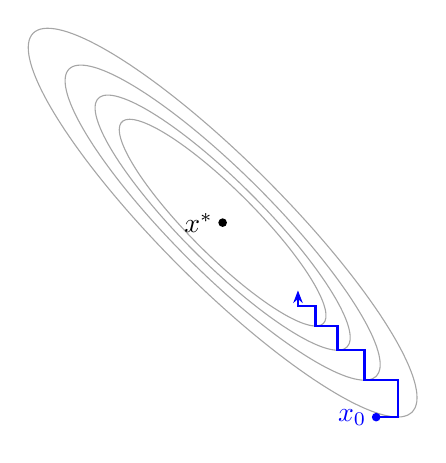
\begin{tikzpicture}[scale=2.6]
        \foreach \ra/\rb in {1.309/0.300,1.061/0.243,0.859/0.197,0.696/0.160}
          \draw[black!35] plot[domain=0:360,samples=72,smooth cycle] ({0.7071*(\ra*cos(\x)+\rb*sin(\x))},{0.7071*(-\ra*cos(\x)+\rb*sin(\x))});
        \draw[blue,thick,->,>={Stealth[length=1.6mm]}]
          (0.750,-0.950)--(0.855,-0.950)--(0.855,-0.769)--(0.693,-0.769)--(0.693,-0.623)--(0.561,-0.623)
          --(0.561,-0.505)--(0.454,-0.505)--(0.454,-0.409)--(0.368,-0.409)--(0.368,-0.331);
        \fill (0,0) circle (0.6pt) node[left] {$x^*$};
        \fill[blue] (0.750,-0.950) circle (0.6pt) node[left] {$x_0$};
      \end{tikzpicture}
    \end{column}
  \end{columns}
\end{frame}

\begin{frame}{Coordinate search: no convergence guarantee}
  \begin{itemize}
    \item It can iterate forever without approaching a stationary point, even with exact line searches.
      A cyclic search along \emph{any} fixed set of linearly independent directions has this defect.
    \item Reason: $-\nabla f_k$ can become nearly perpendicular to the search direction.
      Zoutendijk (3.14) then holds because $\cos\theta_k\to0$, not because $\|\nabla f_k\|\to0$.
    \item When it converges, it is often much slower than steepest descent, and worse as $n$ grows.
    \item Still useful: no gradient, and fast enough if the variables are \alert{loosely coupled}.
  \end{itemize}
  Variants: back-and-forth order $e_1,\dots,e_n,e_{n-1},\dots,e_1,e_2,\dots$;
  a cycle followed by a search along the line joining its first and last points (Hooke--Jeeves).
  \readpp{pp.~229--231.}
\end{frame}

\begin{frame}{Pattern search}
  At $x_k$: a direction set $D_k$ and a step length $\gamma_k$.
  The \textbf{frame} (or stencil) is the set of points $x_k+\gamma_kp_k$, $p_k\in D_k$.
  \begin{itemize}
    \item Some frame point gives a significant decrease: move there; possibly enlarge $\gamma_k$.
    \item None does: stay at $x_k$ and shrink $\gamma_k$ (contract the frame).
    \item $D_k$ may change between iterations, subject to conditions.
  \end{itemize}
  For suitable $D_k$, global convergence can be proved: there is a stationary accumulation point.

  Noise affects the performance and the theory. Nonsmoothness can cause failure in simple examples,
  but convergence on nonsmooth problems is often satisfactory in practice.
\end{frame}

\begin{frame}{Algorithm 9.2 (Pattern search)}
  \algblock{
    Given $\gamma_{\rm tol}$, $\theta_{\max}<1$, and a sufficient decrease function $\rho(t)$,
    increasing, with $\rho(t)/t\to0$ as $t\downarrow0$;\\
    Choose $x_0$, $\gamma_0>\gamma_{\rm tol}$, $D_0$;\\
    \kw{for} $k=1,2,\dots$\\
    \ind \kw{if} $\gamma_k\le\gamma_{\rm tol}$: \kw{stop};\\
    \ind \kw{if} $f(x_k+\gamma_kp_k)<f(x_k)-\rho(\gamma_k)$ for some $p_k\in D_k$\\
    \ind\ind $x_{k+1}\leftarrow x_k+\gamma_kp_k$ for some such $p_k$;\quad
      $\gamma_{k+1}\leftarrow\phi_k\gamma_k$, $\phi_k\ge1$;\\
    \ind \kw{else}\\
    \ind\ind $x_{k+1}\leftarrow x_k$;\quad $\gamma_{k+1}\leftarrow\theta_k\gamma_k$, $0<\theta_k\le\theta_{\max}$;\\
    \kw{end for}
  }
  Evaluate the frame one point at a time and accept the first point with sufficient decrease.
  Choice of $\rho$: $\rho\equiv0$ gives weak theory (Chapter 3); better $\rho(t)=Mt^{3/2}$.
\end{frame}

\begin{frame}{Conditions on the direction set}
  As in Theorem 3.2, some direction must be close to $-\nabla f_k$:
  \begin{equation}
    \cos\theta = \frac{-\nabla f_k^Tp}{\|\nabla f_k\|\,\|p\|}. \tag{9.20}
  \end{equation}
  \begin{block}{Two conditions on $D_k$}
    \vspace{-1ex}
    \begin{align}
      \kappa(D_k) \overset{\text{def}}{=} \min_{v\in\R^n}\max_{p\in D_k}\frac{v^Tp}{\|v\|\,\|p\|} &\ge \delta, \tag{9.21}\\
      \beta_{\min}\le\|p\|\le\beta_{\max} \quad\text{for all } p &\in D_k. \tag{9.22}
    \end{align}
  \end{block}
  Then for any $\nabla f_k$, some $p\in D_k$ satisfies
  \[
    -\nabla f_k^Tp \ge \kappa(D_k)\|\nabla f_k\|\,\|p\| \ge \delta\beta_{\min}\|\nabla f_k\|.
  \]
\end{frame}

\begin{frame}{Direction sets that work}
  \begin{columns}[c]
    \begin{column}{.6\textwidth}
      Coordinate set and simplex set:
      \begin{gather}
        \{e_1,\dots,e_n,-e_1,\dots,-e_n\}, \tag{9.23}\\
        p_i=\tfrac{1}{2n}e-e_i\ (i\le n),\quad p_{n+1}=\tfrac{1}{2n}e. \tag{9.24}
      \end{gather}
      $e=(1,\dots,1)^T$. The simplex set uses only $n+1$ directions.

      \vspace{1ex}
      Coordinate descent is the case $D_k=\{e_i,-e_i\}$: $\kappa(D_k)=0$ (Exercise 9.9).
    \end{column}
    \begin{column}{.38\textwidth}
      \centering
      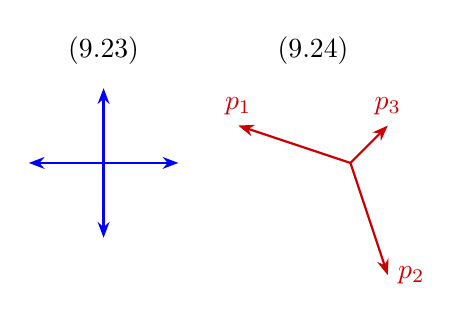
\begin{tikzpicture}[scale=0.95,>={Stealth[length=2mm]}]
        \begin{scope}
          \foreach \x/\y in {1/0,0/1,-1/0,0/-1} \draw[->,thick,blue] (0,0)--(\x,\y);
          \node at (0,1.5) {(9.23)};
        \end{scope}
        \begin{scope}[xshift=3.3cm]
          \draw[->,thick,red!80!black] (0,0)--(-1.5,0.5) node[above] {$p_1$};
          \draw[->,thick,red!80!black] (0,0)--(0.5,-1.5) node[right] {$p_2$};
          \draw[->,thick,red!80!black] (0,0)--(0.5,0.5) node[above] {$p_3$};
          \node at (-0.5,1.5) {(9.24)};
        \end{scope}
      \end{tikzpicture}\\[1ex]
      $n=2$ (cf.\ Figure 9.2)
    \end{column}
  \end{columns}
  \vspace{1ex}
  Other directions may be added, from knowledge of $f$ or from past iterations.
  \readpp{pp.~231--234.}
\end{frame}

\section{\S9.4 A conjugate-direction method}

\begin{frame}{The parallel subspace property}
  \begin{columns}[c]
    \begin{column}{.55\textwidth}
      For $f(x)=\tfrac12x^TAx-b^Tx$ (9.25), $A\succ0$:
      minimize $f$ along two parallel lines $x_1+\alpha p$ and $x_2+\alpha p$.
      Then $x_2^*-x_1^*$ is \alert{conjugate to $p$}.

      \vspace{1ex}
      Proof: $\nabla f(x_i^*)^Tp=0$, so
      \begin{equation}
        0 = (\nabla f(x_1^*)-\nabla f(x_2^*))^Tp = (x_1^*-x_2^*)^TAp. \tag{9.26}
      \end{equation}
      The same holds for parallel affine subspaces $x_i+\mathrm{span}\{p_1,\dots,p_l\}$.
    \end{column}
    \begin{column}{.43\textwidth}
      \centering
      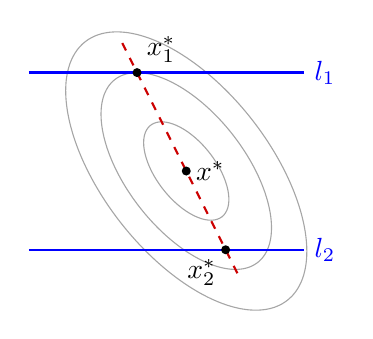
\begin{tikzpicture}[scale=1.25]
        \foreach \ra/\rb in {0.5896/0.2998,1.1791/0.5997,1.6676/0.8481}
          \draw[black!35] plot[domain=0:360,samples=72,smooth cycle] ({0.6157*\ra*cos(\x)+0.7880*\rb*sin(\x)},{-0.7880*\ra*cos(\x)+0.6157*\rb*sin(\x)});
        \draw[blue,thick] (-1.6,1)--(1.2,1) node[right] {$l_1$};
        \draw[blue,thick] (-1.6,-0.8)--(1.2,-0.8) node[right] {$l_2$};
        \draw[red!80!black,thick,dashed] (-0.65,1.3)--(0.55,-1.1);
        \fill (-0.5,1) circle (1.3pt) node[above right] {$x_1^*$};
        \fill (0.4,-0.8) circle (1.3pt) node[below left] {$x_2^*$};
        \fill (0,0) circle (1.3pt) node[right] {$x^*$};
      \end{tikzpicture}\\[.5ex]
      $A=\begin{bmatrix}2&1\\1&1.5\end{bmatrix}$, $p=e_1$ (cf.\ Figure 9.3)
    \end{column}
  \end{columns}
  \vspace{1ex}
  A line search along $x_2^*-x_1^*$ reaches $x^*$ in $\R^2$.
\end{frame}

\begin{frame}{Algorithm 9.3 (DFO method of conjugate directions)}
  \algblock{
    Choose $x_0$; $p_i=e_i$, $i=1,\dots,n$; $x_1\leftarrow$ minimizer of $f$ along $x_0+\alpha p_n$; $k\leftarrow1$;\\
    \kw{repeat} until a convergence test is satisfied\\
    \ind $z_1\leftarrow x_k$;\\
    \ind \kw{for} $j=1,\dots,n$: $\alpha_j$ minimizes $f(z_j+\alpha_jp_j)$; $z_{j+1}\leftarrow z_j+\alpha_jp_j$;\\
    \ind $p_j\leftarrow p_{j+1}$, $j=1,\dots,n-1$;\quad $p_n\leftarrow z_{n+1}-z_1$;\\
    \ind $\alpha_n$ minimizes $f(z_{n+1}+\alpha_np_n)$; $x_{k+1}\leftarrow z_{n+1}+\alpha_np_n$; $k\leftarrow k+1$;\\
    \kw{end repeat}
  }
  \begin{itemize}
    \item Line searches: quadratic interpolation with three values; exact on (9.25).
    \item After iteration $k$, $p_{n-k},\dots,p_n$ are conjugate. Termination after $n-1$ iterations,
      $O(n^2)$ function values, unless a direction becomes zero (Exercise 9.5).
  \end{itemize}
\end{frame}

\begin{frame}{Keeping the directions independent}
  On nonquadratic $f$ the $p_i$ tend to become linearly dependent. Measure conjugacy by
  \begin{equation}
    \hat p_i = \frac{p_i}{\sqrt{p_i^TAp_i}},\qquad |\det(\hat p_1,\dots,\hat p_n)|, \tag{9.27, 9.28}
  \end{equation}
  maximized iff the $p_i$ are conjugate (Powell). Keep (9.28) from decreasing:
  \begin{block}{Procedure 9.4 (Updating the set of directions)}
    $m$: index of the largest decrease $\psi_m=f(x_{m-1})-f(x_m)$ in the inner loop;\\
    $f_1=f(z_1)$, $f_2=f(z_{n+1})$, $f_3=f(2z_{n+1}-z_1)$;\\
    \kw{if} $f_3\ge f_1$ or $(f_1-2f_2+f_3)(f_1-f_2-\psi_m)^2\ge\tfrac12\psi_m(f_1-f_3)^2$\\
    \ind keep $p_1,\dots,p_n$; $x_{k+1}\leftarrow z_{n+1}$;\\
    \kw{else} line search along $\hat p=z_{n+1}-z_1$; replace $p_m$ by $\hat p$. \hfill\readpp{pp.~234--237.}
  \end{block}
\end{frame}

\section{\S9.5 Nelder--Mead method}

\begin{frame}{The Nelder--Mead simplex method (1965)}
  \begin{columns}[c]
    \begin{column}{.5\textwidth}
      Keep $n+1$ points forming a simplex (not the simplex method of Chapter 13), ordered so that
      \[
        f(x_1)\le f(x_2)\le\cdots\le f(x_{n+1}).
      \]
      Centroid of the best $n$, and the line through the worst:
      \[
        \bar x = \frac1n\sum_{i=1}^nx_i,\qquad \bar x(t) = \bar x + t(x_{n+1}-\bar x).
      \]
      $t=-1$ reflect, $-2$ expand, $-\tfrac12$ outside and $\tfrac12$ inside contraction.
    \end{column}
    \begin{column}{.48\textwidth}
      \centering
      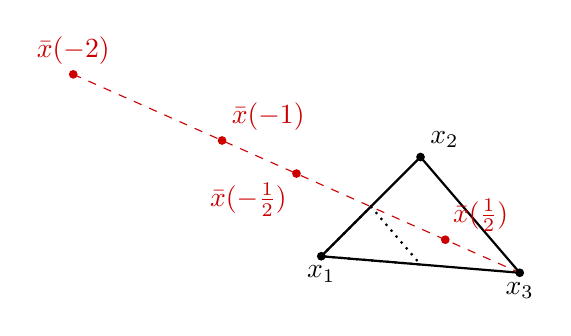
\begin{tikzpicture}[scale=1.05]
        \coordinate (x1) at (0,0); \coordinate (x2) at (1.2,1.2); \coordinate (x3) at (2.4,-0.2);
        \draw[thick] (x1)--(x2)--(x3)--cycle;
        \draw[dotted,thick] (0,0)--(0.6,0.6)--(1.2,-0.1)--cycle;
        \draw[red!80!black,dashed] (-3,2.2)--(2.4,-0.2);
        \fill[red!80!black] (-1.2,1.4) circle (1.5pt) node[above right] {$\bar x(-1)$};
        \fill[red!80!black] (-3,2.2) circle (1.5pt) node[above] {$\bar x(-2)$};
        \fill[red!80!black] (-0.3,1.0) circle (1.5pt) node[below left] {$\bar x(-\frac12)$};
        \fill[red!80!black] (1.5,0.2) circle (1.5pt) node[above right=-1pt] {$\bar x(\frac12)$};
        \fill (x1) circle (1.5pt) node[below] {$x_1$};
        \fill (x2) circle (1.5pt) node[above right] {$x_2$};
        \fill (x3) circle (1.5pt) node[below] {$x_3$};
      \end{tikzpicture}\\[.5ex]
      $n=2$; dotted: shrunken simplex (cf.\ Figure 9.4)
    \end{column}
  \end{columns}
\end{frame}

\begin{frame}{Procedure 9.5 (One step of Nelder--Mead)}
  \algblock{
    $f_{-1}=f(\bar x(-1))$;\\
    \kw{if} $f(x_1)\le f_{-1}<f(x_n)$: replace $x_{n+1}$ by $\bar x(-1)$; \hfill (reflect)\\
    \kw{else if} $f_{-1}<f(x_1)$: $f_{-2}=f(\bar x(-2))$; \hfill (expand)\\
    \ind replace $x_{n+1}$ by $\bar x(-2)$ if $f_{-2}<f_{-1}$, else by $\bar x(-1)$;\\
    \kw{else} ($f_{-1}\ge f(x_n)$): \hfill (contract)\\
    \ind \kw{if} $f_{-1}<f(x_{n+1})$: \kw{if} $f(\bar x(-\tfrac12))\le f_{-1}$, replace $x_{n+1}$ by $\bar x(-\tfrac12)$; \hfill (outside)\\
    \ind \kw{else}: \kw{if} $f(\bar x(\tfrac12))<f(x_{n+1})$, replace $x_{n+1}$ by $\bar x(\tfrac12)$; \hfill (inside)\\
    \ind if the contraction fails, shrink: $x_i\leftarrow\tfrac12(x_1+x_i)$, $i=2,\dots,n+1$.
  }
  The values $t=-1,-2,-\tfrac12,\tfrac12$ are standard; other choices are possible.
\end{frame}

\begin{frame}{Nelder--Mead in practice}
  \begin{itemize}
    \item Unless a shrink step occurs, the average function value over the vertices
      \begin{equation}
        \frac1{n+1}\sum_{i=1}^{n+1}f(x_i) \tag{9.29}
      \end{equation}
      decreases at every step (Exercise 9.11). For convex $f$, the shrink step does not increase it (Exercise 9.12).
    \item Practical performance is often reasonable, but the method can \alert{stagnate at nonoptimal points}.
      Remedy: restart when stagnation is detected (Kelley).
    \item Convergence theory is limited (Kelley; Lagarias et al.).
    \item (Not in the book.) McKinnon (1998): a smooth, strictly convex function in $\R^2$
      on which Nelder--Mead converges to a nonstationary point.
  \end{itemize}
  \readpp{pp.~238--240.}
\end{frame}

\section{\S9.6 Implicit filtering}

\begin{frame}{Implicit filtering: the idea}
  For noisy $f=h+\phi$ as in (9.2):
  \begin{itemize}
    \item Steepest descent with an Armijo line search (Chapter 3), using the central difference $\nabla_\eps f$ (9.3)
      with an $\eps$ that is \alert{not} particularly small.
    \item Works best when the noise decreases near the solution, for example when we control
      the solver tolerance or the number of simulation trials.
    \item Decrease $\eps$ systematically, but more slowly than the noise, so that $\nabla_\eps f$ stays accurate (Lemma 9.1).
    \item For each $\eps$: backtracking line search on $-\nabla_\eps f$.
      If it fails after $a_{\max}$ backtracks, or if $\|\nabla_\eps f\|\le\eps$, go to the next, smaller $\eps$.
  \end{itemize}
\end{frame}

\begin{frame}{Algorithm 9.6 (Implicit filtering)}
  \algblock{
    Choose $\{\eps_k\}\downarrow0$, Armijo parameters $c,\rho\in(0,1)$, $a_{\max}$; $k\leftarrow1$; $x\leftarrow x_0$;\\
    \kw{repeat}\\
    \ind \kw{repeat}\\
    \ind\ind compute $f(x)$ and $\nabla_{\eps_k}f(x)$;\\
    \ind\ind \kw{if} $\|\nabla_{\eps_k}f(x)\|\le\eps_k$: leave the inner loop;\\
    \ind\ind find the smallest $m\in\{0,\dots,a_{\max}\}$ with\\
    \ind\ind\ind $f\bigl(x-\rho^m\nabla_{\eps_k}f(x)\bigr)\le f(x)-c\rho^m\|\nabla_{\eps_k}f(x)\|^2$;\\
    \ind\ind \kw{if} there is none: leave the inner loop; \kw{else} $x\leftarrow x-\rho^m\nabla_{\eps_k}f(x)$;\\
    \ind \kw{end repeat}\\
    \ind $x_k\leftarrow x$; $k\leftarrow k+1$;\\
    \kw{until} a termination test is satisfied \hfill (inner loop = Algorithm 3.1 + a test)
  }
\end{frame}

\begin{frame}{Theorem 9.2: convergence of implicit filtering}
  \begin{block}{Theorem 9.2}
    Suppose that $\nabla^2h$ is Lipschitz continuous, that Algorithm 9.6 generates an infinite sequence $\{x_k\}$, and that
    \[
      \lim_{k\to\infty}\Bigl(\eps_k^2+\frac{\eta(x_k;\eps_k)}{\eps_k}\Bigr) = 0.
    \]
    Suppose also that all but finitely many inner loops terminate with $\|\nabla_{\eps_k}f(x_k)\|\le\eps_k$.
    Then all limit points of $\{x_k\}$ are stationary.
  \end{block}
  \textbf{Proof.} $\eps_k\downarrow0$ gives $\nabla_{\eps_k}f(x_k)\to0$.
  The right-hand side of (9.5) tends to 0, so $\nabla h(x_k)\to0$. \hfill$\square$

  \vspace{1ex}
  The noise must vanish faster than $\eps_k$. Refinement: use $\nabla_{\eps_k}f$ in quasi-Newton updates.
  \readpp{pp.~240--242.}
\end{frame}

\section{Chapter 9: summary}

\begin{frame}{Numerical example: Rosenbrock's function (2.22)}
  Starting point $(-1.2,1)$; SciPy 1.17, default settings with tight tolerances. (Not in the book.)

  \vspace{1ex}
  \centering
  \renewcommand{\arraystretch}{1.1}
  \begin{tabular}{llrl}
    \toprule
    Method & Section & $f$ evaluations & $\|x-x^*\|$\\
    \midrule
    Nelder--Mead & \S9.5 & 219 & $2\times10^{-9}$\\
    Powell (conjugate directions) & \S9.4 & 792 & $5\times10^{-14}$\\
    Pattern search (9.23), $\rho(t)=10^{-4}t^{3/2}$ & \S9.3 & 19\,182 & $9\times10^{-6}$\\
    COBYLA (linear models) & \S9.2 & 18\,294 & $3\times10^{-7}$\\
    BFGS + forward differences & \S9.1 & 120 & $1\times10^{-5}$\\
    BFGS + exact gradient & Ch.~6 & 41 (+41 $\nabla f$) & $1\times10^{-12}$\\
    \bottomrule
  \end{tabular}

  \vspace{1ex}
  \raggedright
  Linear models and fixed directions are slow on a curved valley. Finite differences are cheap
  but stop at about $\sqrt u$ accuracy.
\end{frame}

\begin{frame}{Chapter 9 in one table}
  \centering
  \renewcommand{\arraystretch}{1.1}
  \begin{tabular}{lll}
    \toprule
    Method & Uses & Theory\\
    \midrule
    FD + gradient & tight cluster & fails if $\eta\gg\eps$ (9.5)\\
    Model-based (9.1) & interpolation + TR & geometry of $Y$\\
    Minimum change (9.19) & $2n+1$ points, $O(n^3)$ & NEWUOA\\
    Coordinate search & $\pm e_i$, cyclic & may not converge\\
    Pattern search (9.2) & frame, $\kappa(D_k)\ge\delta$ & stationary limit point\\
    Conjugate directions (9.3) & parallel subspaces & finite on quadratics\\
    Nelder--Mead (9.5) & simplex reflection & limited; can stagnate\\
    Implicit filtering (9.6) & FD with shrinking $\eps_k$ & Theorem 9.2\\
    \bottomrule
  \end{tabular}
\end{frame}

\begin{frame}{Three results to carry forward}
  \begin{enumerate}
    \item \textbf{Noise sets the difference interval.}
      Error $\le L_h\eps^2+\eta/\eps$ (Lemma 9.1): with noise, small $\eps$ is harmful.
    \item \textbf{Model-based DFO is trust-region optimization with an interpolated model.}
      The new ingredient is keeping the interpolation set well poised: $\delta(Y)$, Lagrange functions.
    \item \textbf{Directions must cover all of $\R^n$.}
      Pattern search converges because $\kappa(D_k)\ge\delta>0$; coordinate descent has $\kappa=0$.
  \end{enumerate}
  \vspace{1ex}
  Use DFO only for small $n$, and only when derivatives (Chapter 8) are truly unavailable.
\end{frame}

\begin{frame}{Homework {\normalsize (problems 5--6 are not in the book)}}
  \begin{enumerate}
    \item Exercise 9.1: prove Lemma 9.1.
    \item Exercise 9.2: count the interpolation conditions; vertices and edge midpoints of a simplex.
    \item Exercise 9.7: find the quadratic that interpolates the six given data points.
    \item Exercise 9.9: show that $\kappa(\{e_i,-e_i\})=0$.
    \item Implement Algorithm 9.2 with the sets (9.23) and (9.24). Run it on Rosenbrock (2.22) from $(-1.2,1)$
      and compare the number of evaluations.
    \item Add uniform noise of size $10^{-4}$ to Rosenbrock. Compare Nelder--Mead with BFGS using forward differences,
      $\eps=\sqrt u$ and $\eps=10^{-2}$.
  \end{enumerate}
\end{frame}

\end{document}
